\clearpage\section*{Appendix A. Test a narrower 2016 window: $\pm2u$}
\label{sec:windowappendix}

\textbf{The finding.} Reducing the 2016 MC fit and GP-training exclusion from $\pm3.5u$ to $\pm2u$ lowers most conditional observed profile limits. However, it also reduces the fitted response to an injected full MC signal. In the five tested injections, the narrower window recovers 87.7--92.2\% of the added selected yield, compared with 99.8--100.1\% for the main window. Its smaller raw fit uncertainty therefore does not establish an improvement in signal sensitivity.

\textbf{A controlled window comparison.} Both choices use the same neighboring MC template, $u=(m_{\rm rec}-c)/s$, and the same interpolated core center and width. Only the interval changes. For the comparison, bins with centers satisfying $|u|\le2$ enter the signal likelihood and are excluded from GP training. All other bins enter training. There is no separate extra exclusion. The full selected template normalization, GP kernel settings and inherited coupling conversion are retained; the GP mean and covariance are recomputed for the new sidebands.
\begin{center}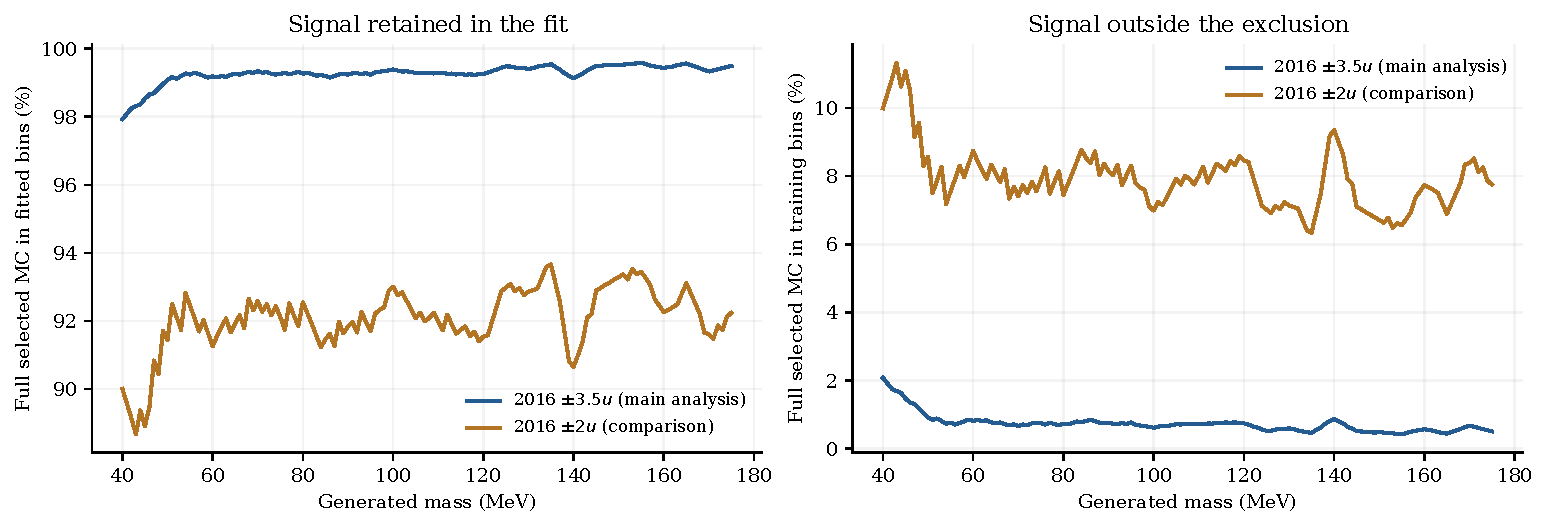
\includegraphics[width=\linewidth,height=2.65in,keepaspectratio]{../figures/window_geometry.pdf}\end{center}
{\small\refstepcounter{figure}\textbf{Figure \thefigure. How to read the figure.} Blue is the main $\pm3.5u$ prescription; gold is $\pm2u$. Left: full selected MC probability in the actual analysis bins used for fitting. Right: probability in the GP-training bins. Bin membership follows bin centers, so the plotted fractions include the finite analysis binning. These are geometric fractions, not detector efficiencies or fitted recovery fractions.}\par\medskip

The narrower fitted bins contain 88.68--93.66\% of the full selected signal over 40--175 MeV, compared with 97.93--99.58\% in the main window. Consequently, 6.34--11.32\% can enter training rather than 0.42--2.07\%. The tail probability is retained in the injections. It is never dropped or renormalized into the fitted interval.

\begin{center}\small\begin{tabular}{rrrrr}\toprule
Mass [MeV] & Window & Actual fit interval [MeV] & Fit bins & MC fraction [\%]\\\midrule
69 & $\pm3.5u$ & 59.50--78.25 & 75 & 99.29\\
69 & $\pm2u$ & 63.50--74.25 & 43 & 92.32\\
91 & $\pm3.5u$ & 78.50--103.00 & 98 & 99.27\\
91 & $\pm2u$ & 83.75--97.75 & 56 & 91.97\\
\bottomrule\end{tabular}\end{center}
The main-body results remain the $\pm3.5u$ analysis. This appendix tests an alternative; it does not replace that prescription.

\clearpage\section*{Appendix A.1. The 2016 observed scan}
The two windows are evaluated at the same 136 hypotheses, 40--175 MeV in 1 MeV steps. Limits continue to refer to the full selected MC yield. The signal shape itself is identical in the two fits.
\begin{center}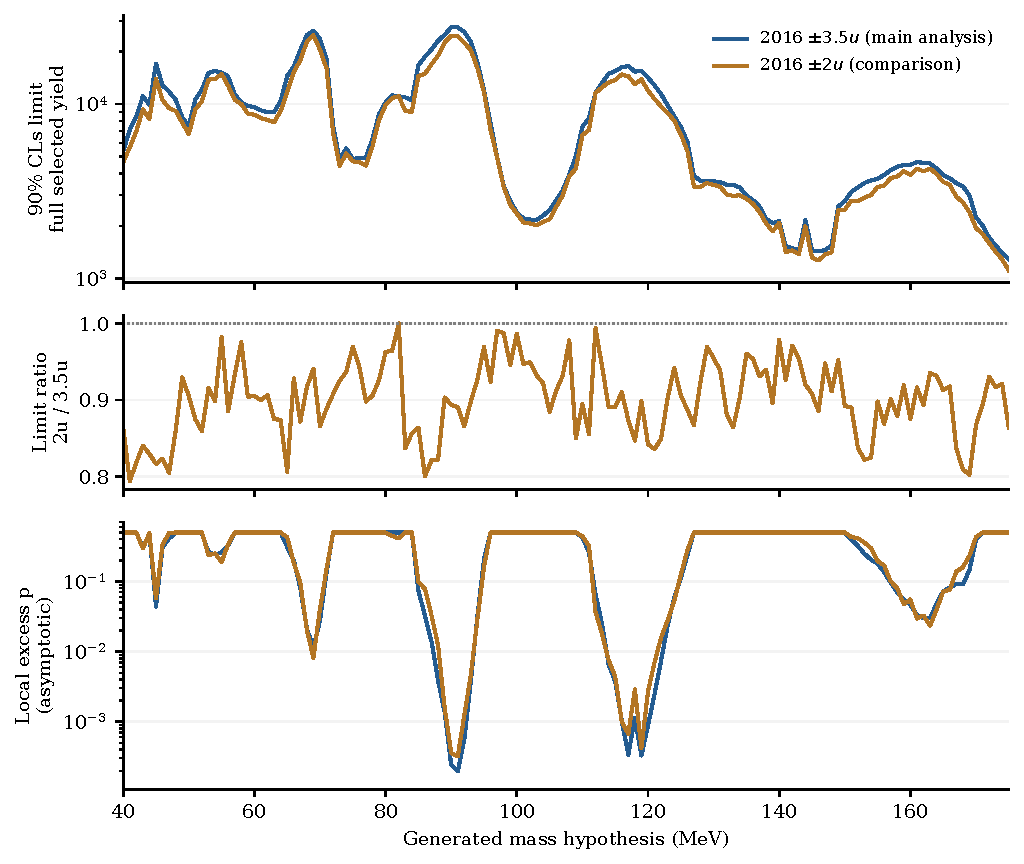
\includegraphics[width=\linewidth,height=4.55in,keepaspectratio]{../figures/window_2016.pdf}\end{center}
{\small\refstepcounter{figure}\textbf{Figure \thefigure. How to read the figure.} Top: conditional observed 90\% profile-$CL_s$ upper limits for the two windows. Middle: the $\pm2u$ limit divided by the $\pm3.5u$ limit at the same mass. Bottom: fixed-mass local asymptotic excess probabilities. These curves use the likelihood and conversion defined in the main text; they are not full-scan toy-calibrated limits or global probabilities.}\par\medskip

The median limit change is $-9.64\%$, with a range of $-20.63\%$ at 41 MeV to $+0.05\%$ at 82 MeV. At 91 MeV, the strongest local feature under both choices, the fitted yield changes from $20{,}201\pm5{,}699$ to $17{,}815\pm5{,}221$ events. The upper limit falls from 27,505 to 24,507 events, while the local asymptotic probability increases from 0.000196 to 0.000321 ($Z=3.55$ to 3.41).

At the other previously selected region, 69 MeV, the fitted yield changes from $16{,}791\pm7{,}371$ to $16{,}115\pm6{,}705$ events, the upper limit from 26,285 to 24,739 events, and the local asymptotic probability from 0.01136 to 0.00812. These fixed-mass comparisons keep the two earlier examples; they do not select a new pair of independent excesses.

\clearpage\section*{Appendix A.2. Propagate only the 2016 window change}
This comparison starts from the final main-body combination: 2015 Gaussian, 2016 neighboring MC and 2021 neighboring MC. The 2021 interval remains $[-4,+3]u$. Campaign availability, observations, full signal probabilities and coupling conversion are identical; only the 2016 fit/exclusion changes.
\begin{center}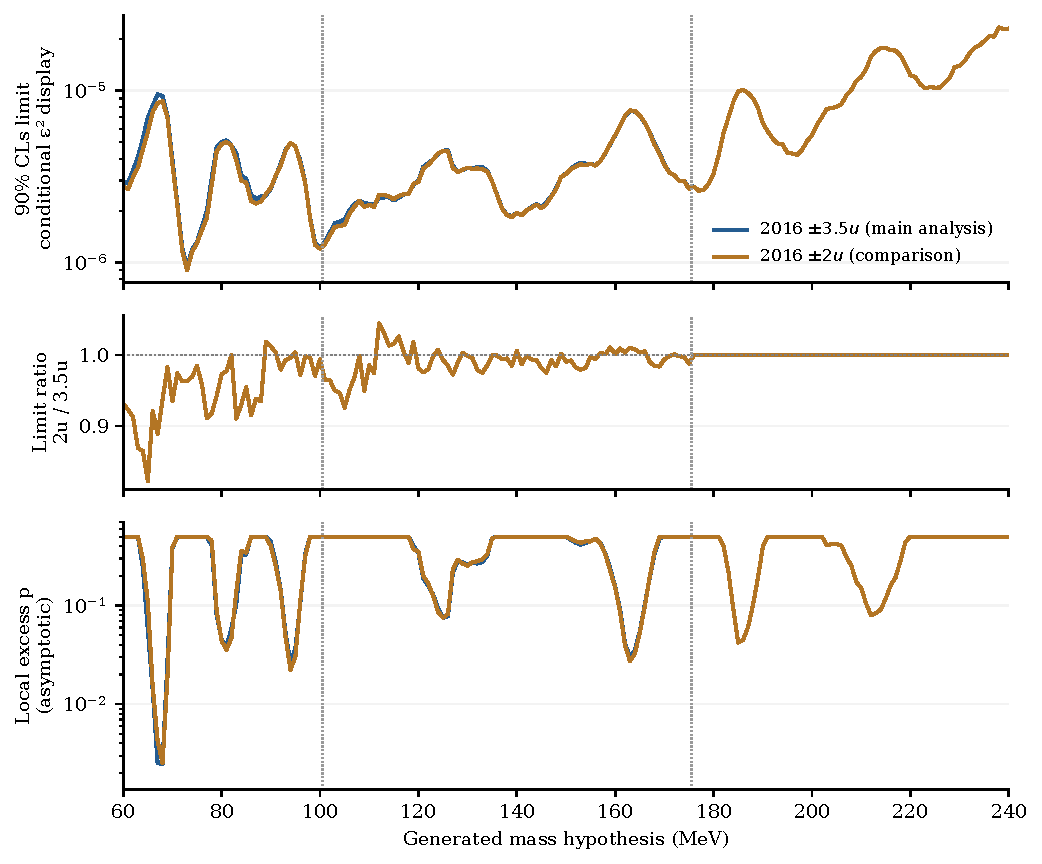
\includegraphics[width=\linewidth,height=4.55in,keepaspectratio]{../figures/window_combined.pdf}\end{center}
{\small\refstepcounter{figure}\textbf{Figure \thefigure. How to read the figure.} Top: the conditional coupling-limit display for the main combination and the combination with 2016 narrowed to $\pm2u$. Middle: their ratio. Bottom: local asymptotic excess probabilities from the joint common-signal likelihood. Vertical dotted lines mark the ends of 2015 and 2016 participation. Above 175 MeV only 2021 contributes, so both curves coincide exactly. No new global probability or efficiency correction is inferred.}\par\medskip

Over 60--175 MeV, where 2016 contributes, the combined upper limit changes by a median $-1.36\%$. The range is $-17.83\%$ at 65 MeV to $+4.49\%$ at 112 MeV. The effect is smaller than the typical 2016-only shift because the common signal parameter must also describe the other included campaigns.

The strongest combined local feature stays at 68 MeV: $p_0$ changes only from 0.002475 to 0.002539 ($Z=2.810$ to 2.802). The narrower-window scan remains a conditional profile comparison. The main-body selected-point rank calibration used the wider 2016 prescription and is not transferred to this alternative.

\clearpage\section*{Appendix A.3. Does the narrower window recover the signal?}

At 60, 69, 91, 100 and 160 MeV, 200 paired experiments add the same full MC signal to the same fixed GP-mean background for both windows. The expected selected yield is $A=3s_0$, where $s_0$ is the wider-window MC fit's Hessian error on the fixed background mean. Each stored-bin and outside-support signal category is Poisson sampled. Background-only and signal-injected fits share their background draw; neither the observed spectrum nor a fitted null bias determines the injected yield.

The response below is $R=\langle\Ah_{s+b}-\Ah_b\rangle/A$. Pairing removes the background-only mean from this response measurement; no correction is applied to the observed fits.
\begin{center}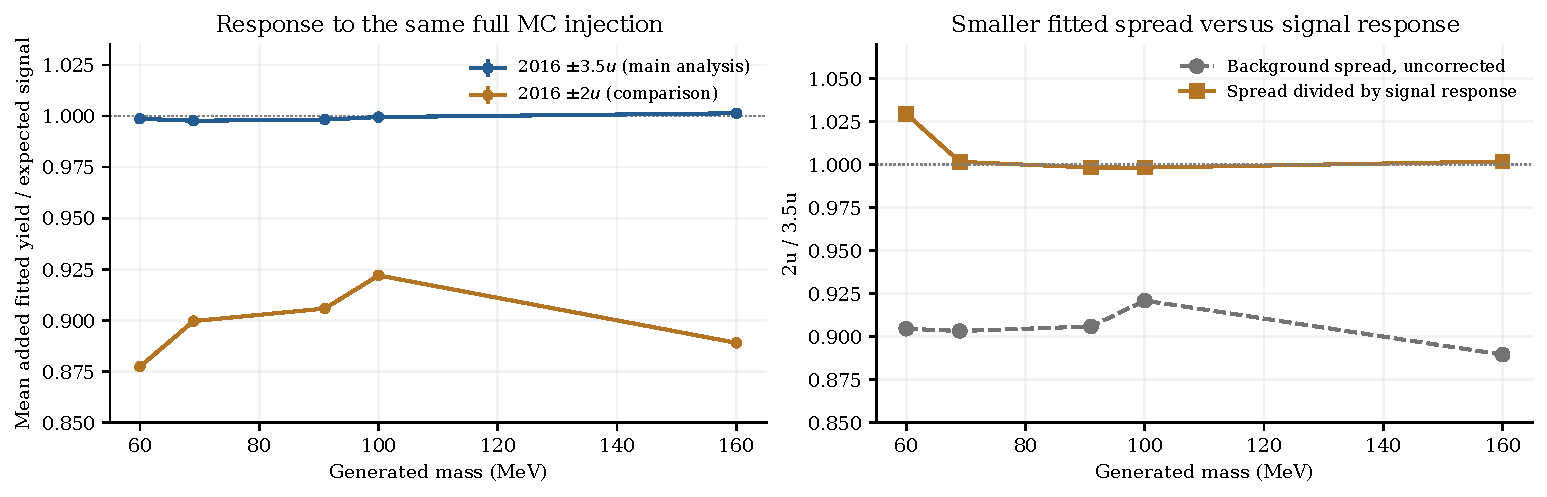
\includegraphics[width=\linewidth,height=2.65in,keepaspectratio]{../figures/window_response.pdf}\end{center}
{\small\refstepcounter{figure}\textbf{Figure \thefigure. How to read the figure.} Left: response to the same expected full selected signal; error bars are Monte Carlo standard errors of the paired mean. Right: the ratio of background-toy fitted-yield spreads, before and after dividing each spread by its response. The ratios are descriptive point estimates from 200 paired experiments; their few-percent differences are not precise sensitivity improvements. Neither panel measures coverage.}\par\medskip

The narrower response is 0.877--0.922, while the wider response is 0.998--1.001. Dividing the background fitted-yield spread by the response gives narrow/wide ratios of 0.998--1.030. Thus the smaller raw fitted spread is largely offset by the reduced response. Together with the extra signal in training bins, this is consistent with increased signal absorption by the background estimate. It supports retaining $\pm3.5u$ as the main choice in this bounded comparison.

\textbf{Local background check.} Both windows also use the same 1,000 fixed-source null draws at 69 and 91 MeV. At 91 MeV, $\pm2u$ has 1 exceedance, rank $2/1001=0.0020$, and a 95\% exact binomial interval [0.000025, 0.00556]; $\pm3.5u$ has 3, rank 0.0040, with [0.00062, 0.00874]. At 69 MeV the counts are 3 and 5, with ranks 0.0040 and 0.0060 and intervals [0.00062, 0.00874] and [0.00163, 0.01163]. These sparse, paired tails do not establish a significant difference between windows. The positive mean null root at 91 MeV remains: 0.601 versus 0.656.

\textbf{Record and scope.} The appendix adds 252 observed fits and 6,000 toy fits, reusing 2,000 matching main-body null rows. Complete signed yields, Hessian errors, pulls, realized signal partitions, pairing hashes and probability intervals are under \path{results/window_comparison}. This is a five-mass, one-strength, fixed-source response check, not an independent coverage validation or a new calibrated upper-limit construction. Rebuild the appendix with \path{rebuild_appendix.sh}; the parent numerical records remain unchanged.
